% Figure -- designable vs non-designable backbones (Ca cartoons).
% \input{} from Ch3 (sec:eval-protein, after the Designability paragraph).
% Source: figures/scripts/fig_ch3_designability.py
\begin{figure}[tbp]
\centering
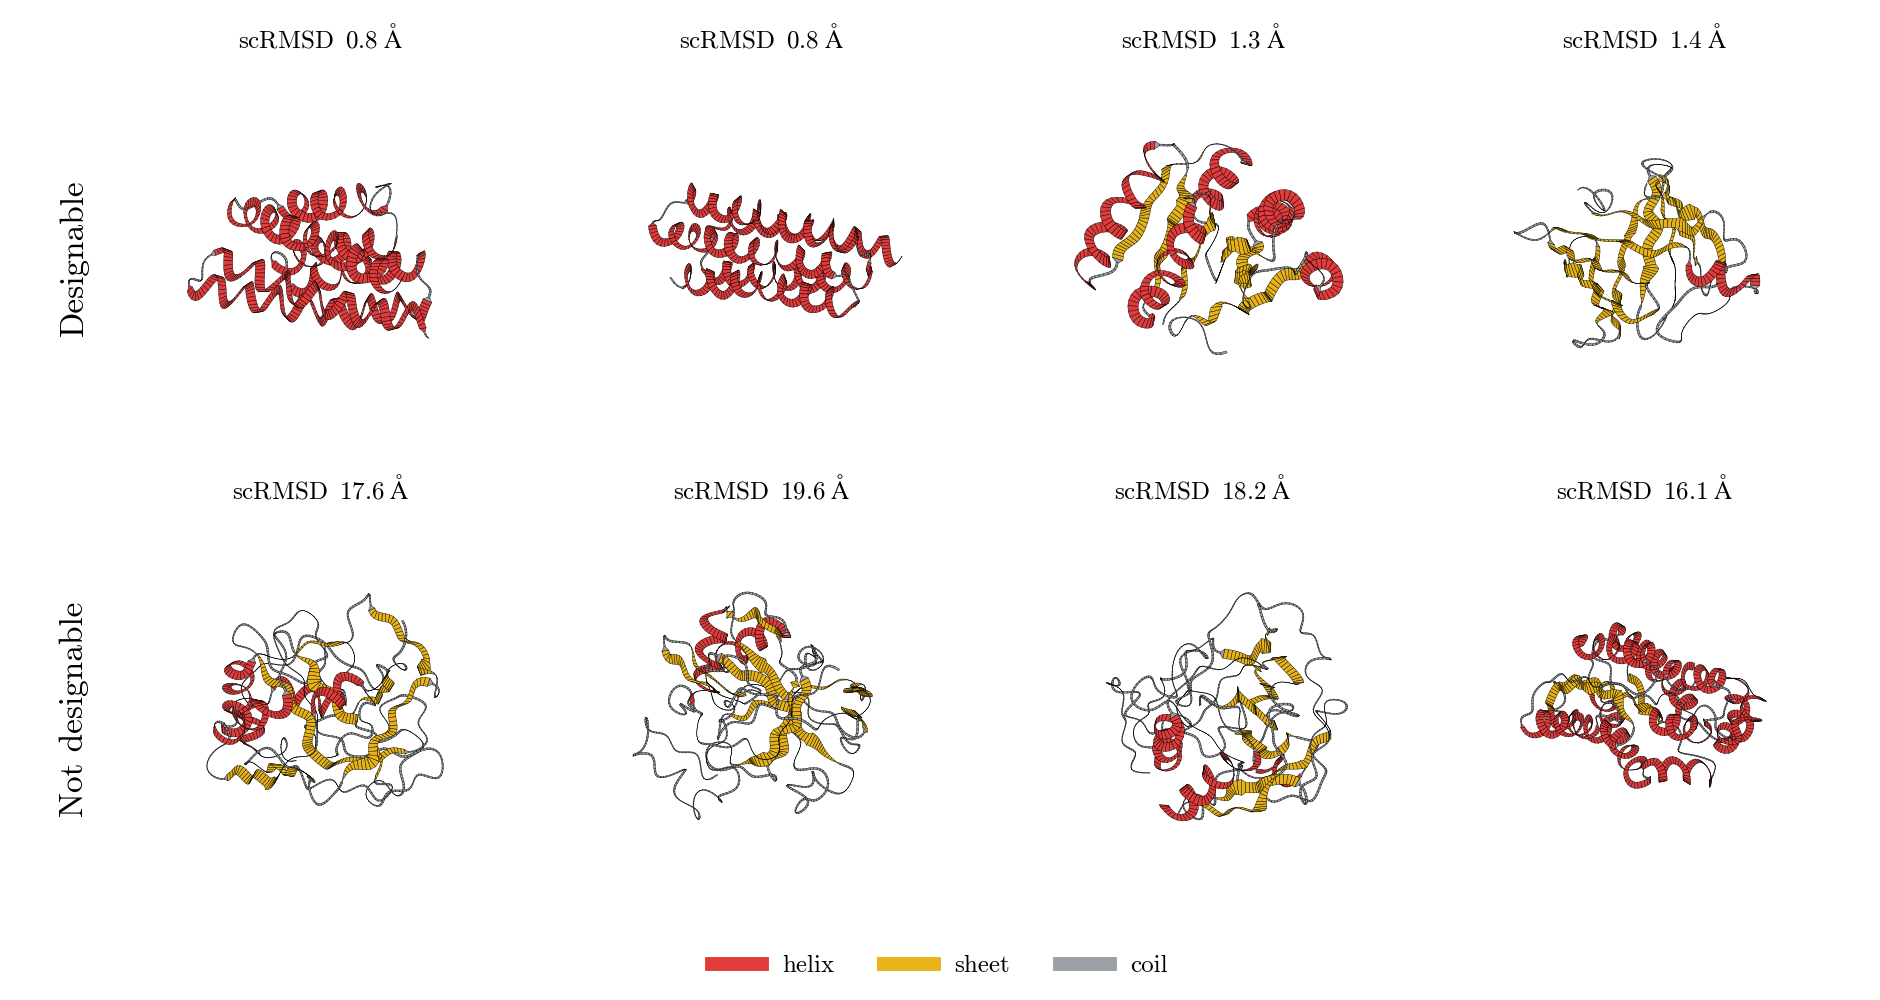
\includegraphics[width=\textwidth]{figures/fig_ch3_designability.png}
\caption{Designable versus non-designable backbones. Designable ones (top, scRMSD${<}2$\,\AA{}) re-fold to their generated shape; non-designable ones (bottom, $16$--$20$\,\AA{}) do not. The two right-hand designable examples are $\beta$-rich, not easy helices. From our PDB models at 1.3M steps (\S\ref{sec:proteina-anatomy}).}
\label{fig:designability}
\end{figure}
